% !TEX root = ./../main.tex
\chapter{Summary and conclusions}
\label{chap:conclusions}
% Brevemento cosa ho fatto
% Risultati più importanti:
% abbiamo definito un protocollo per il calcolo delle buche di andata e ritorno separatamente, il fatto che i percorsi siano diversi. Prospettive di sviluppo: vedere come cambia tirando giù altri ligandi, CV diversi nella speranza di trovare meccanismi alternativi e vantaggiosi, capire  se è favorito o meno dalla presenta di altre NP nella membrana
%
% Convinti che martini STD rimane qualitativamente indispensabile ma quantitativamente insufficente per via dell'int elettrostatoca: usare PME PW. Efficienza tra i due modelli.
%
% La differenza tra Random e striped rimane confermato: studiare ligandi diversi, NP con dimensioni più grandi che permattano di giocare con i diversi arrangement.

In this work I have approached the study of the interaction between \acp{AuNP} and biological membranes by computational means. The molecular mechanisms of interaction between these synthetic \acp{NP} and biological membranes are, on the one hand, hard to be identified experimentally and, on the other hand, fundamental to be able to design \acp{NP} with a controlled interaction with cell membranes.
\begin{figure}[!ht]
	\center
	\subfloat[Striped arranged \acs{NP}]{%
		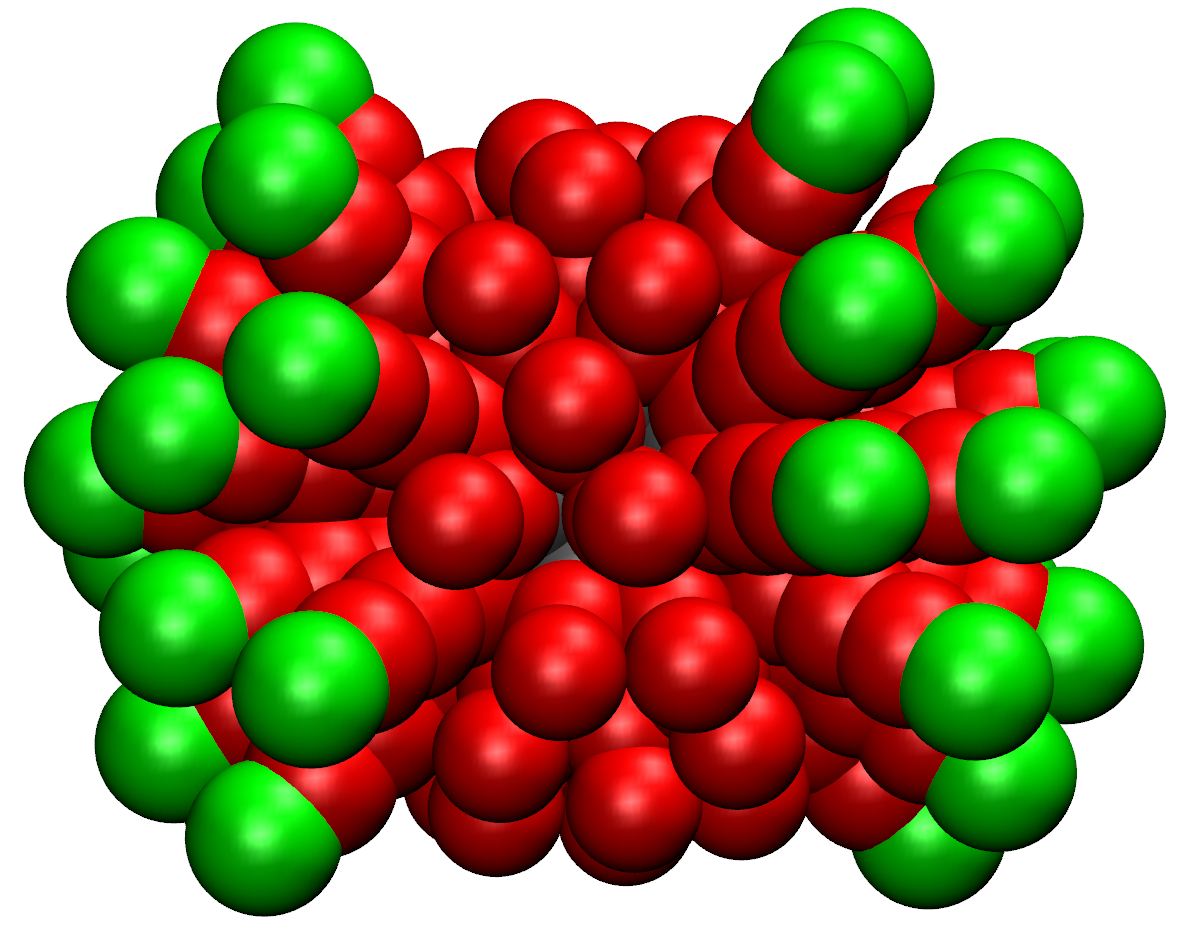
\includegraphics[width=0.25\textwidth]{./img/coatings/striped}%
	}\qquad\qquad%
	\subfloat[Random arranged \acs{NP}]{%
		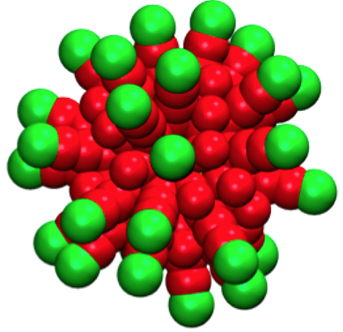
\includegraphics[width=0.25\textwidth]{./img/coatings/random11}%
	}\\%
	\subfloat[\acs{NP} in hydrophobic contact]{%
		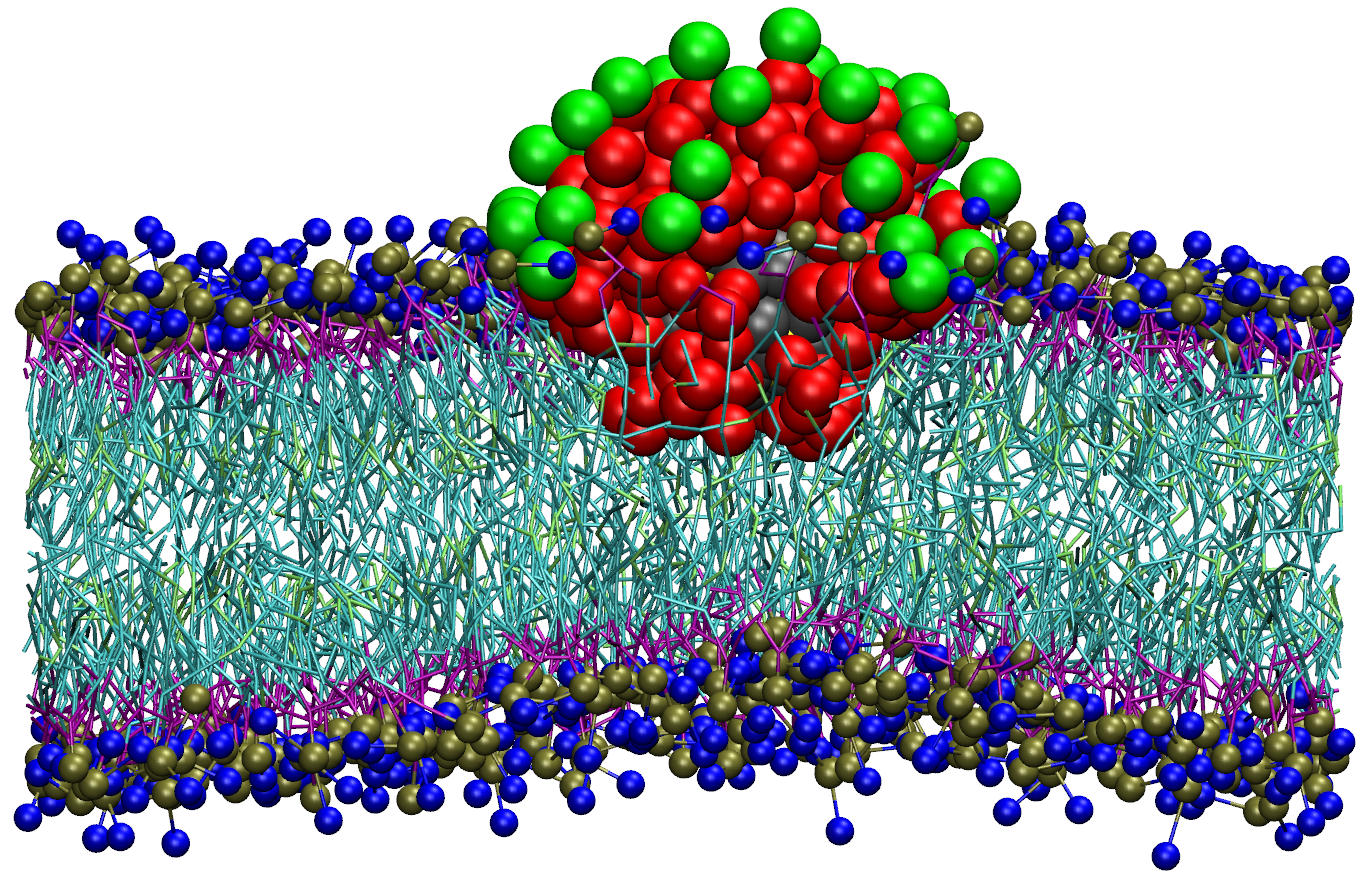
\includegraphics[width=0.7\textwidth]{./img/NPMembrane}%
	}%
	\caption{(a) The striped arranged \acs{NP}. (b) The random arranged \acs{NP}. (c) Striped \acs{NP} interacting with the model lipid membrane. In red the hydrophobic beads and in green the negatively charged beads of the \acs{NP} ligands. In gray the sulfur atoms of the \acs{NP}'s core. In blue the choline groups, in tan the phosphate groups and in violet the glycerol groups of the lipid heads. The lipid tails are shown as cyan colored stick. Beads of the water solvent are not shown for clarity.}
	\label{fig:NPSummary}
\end{figure}

In particular, I focused on the interaction between monolayer--protected, anionic \ac{AuNP} and model lipid bilayers. The surface charge of the ligand--protected \ac{NP}s makes them water--soluble, but it also affects their interaction with lipid membranes. Our simulations aimed at clarifying the role played by electrostatic during the passive \ac{NP}--membrane interaction. In particular, we have performed unbiased \ac{MD} simulations and free energy calculations using models that differ in resolution and in the way they treat electrostatic interactions. We compared the outcomes of the different models with respect to a. the energetics of the \ac{NP}--membranes interactions and b. the molecular mechanisms involved.

In the following, we summarize the main results we obtained in relation to each of the objectives listed in the Introduction. We will also describe possible future research perspectives.

\begin{enumerate}[label=\itshape\roman*.,listparindent=1em]
	\item \textbf{\textsf{Is the binding of anionic \acp{NP} to zwitterionic lipid membranes favorable from an energetic point of view? Yes it is.}}\\With advanced sampling techniques \textit{I estimated the free energy profiles of one charged ligand translocation across the lipid membrane}, as shown in figure~(\ref{fig:coglionazzo}). For the striped (\acs{MUS}:\acs{OT} $1$:$1$) \ac{NP} I have found that both the anchoring and dis--anchoring processes (forward and backward in figure~(\ref{fig:coglionazzo}), respectively) are characterized by extremely large free energy barriers: $100$~kJ/mol.%
\begin{figure}[ht]
	\center
	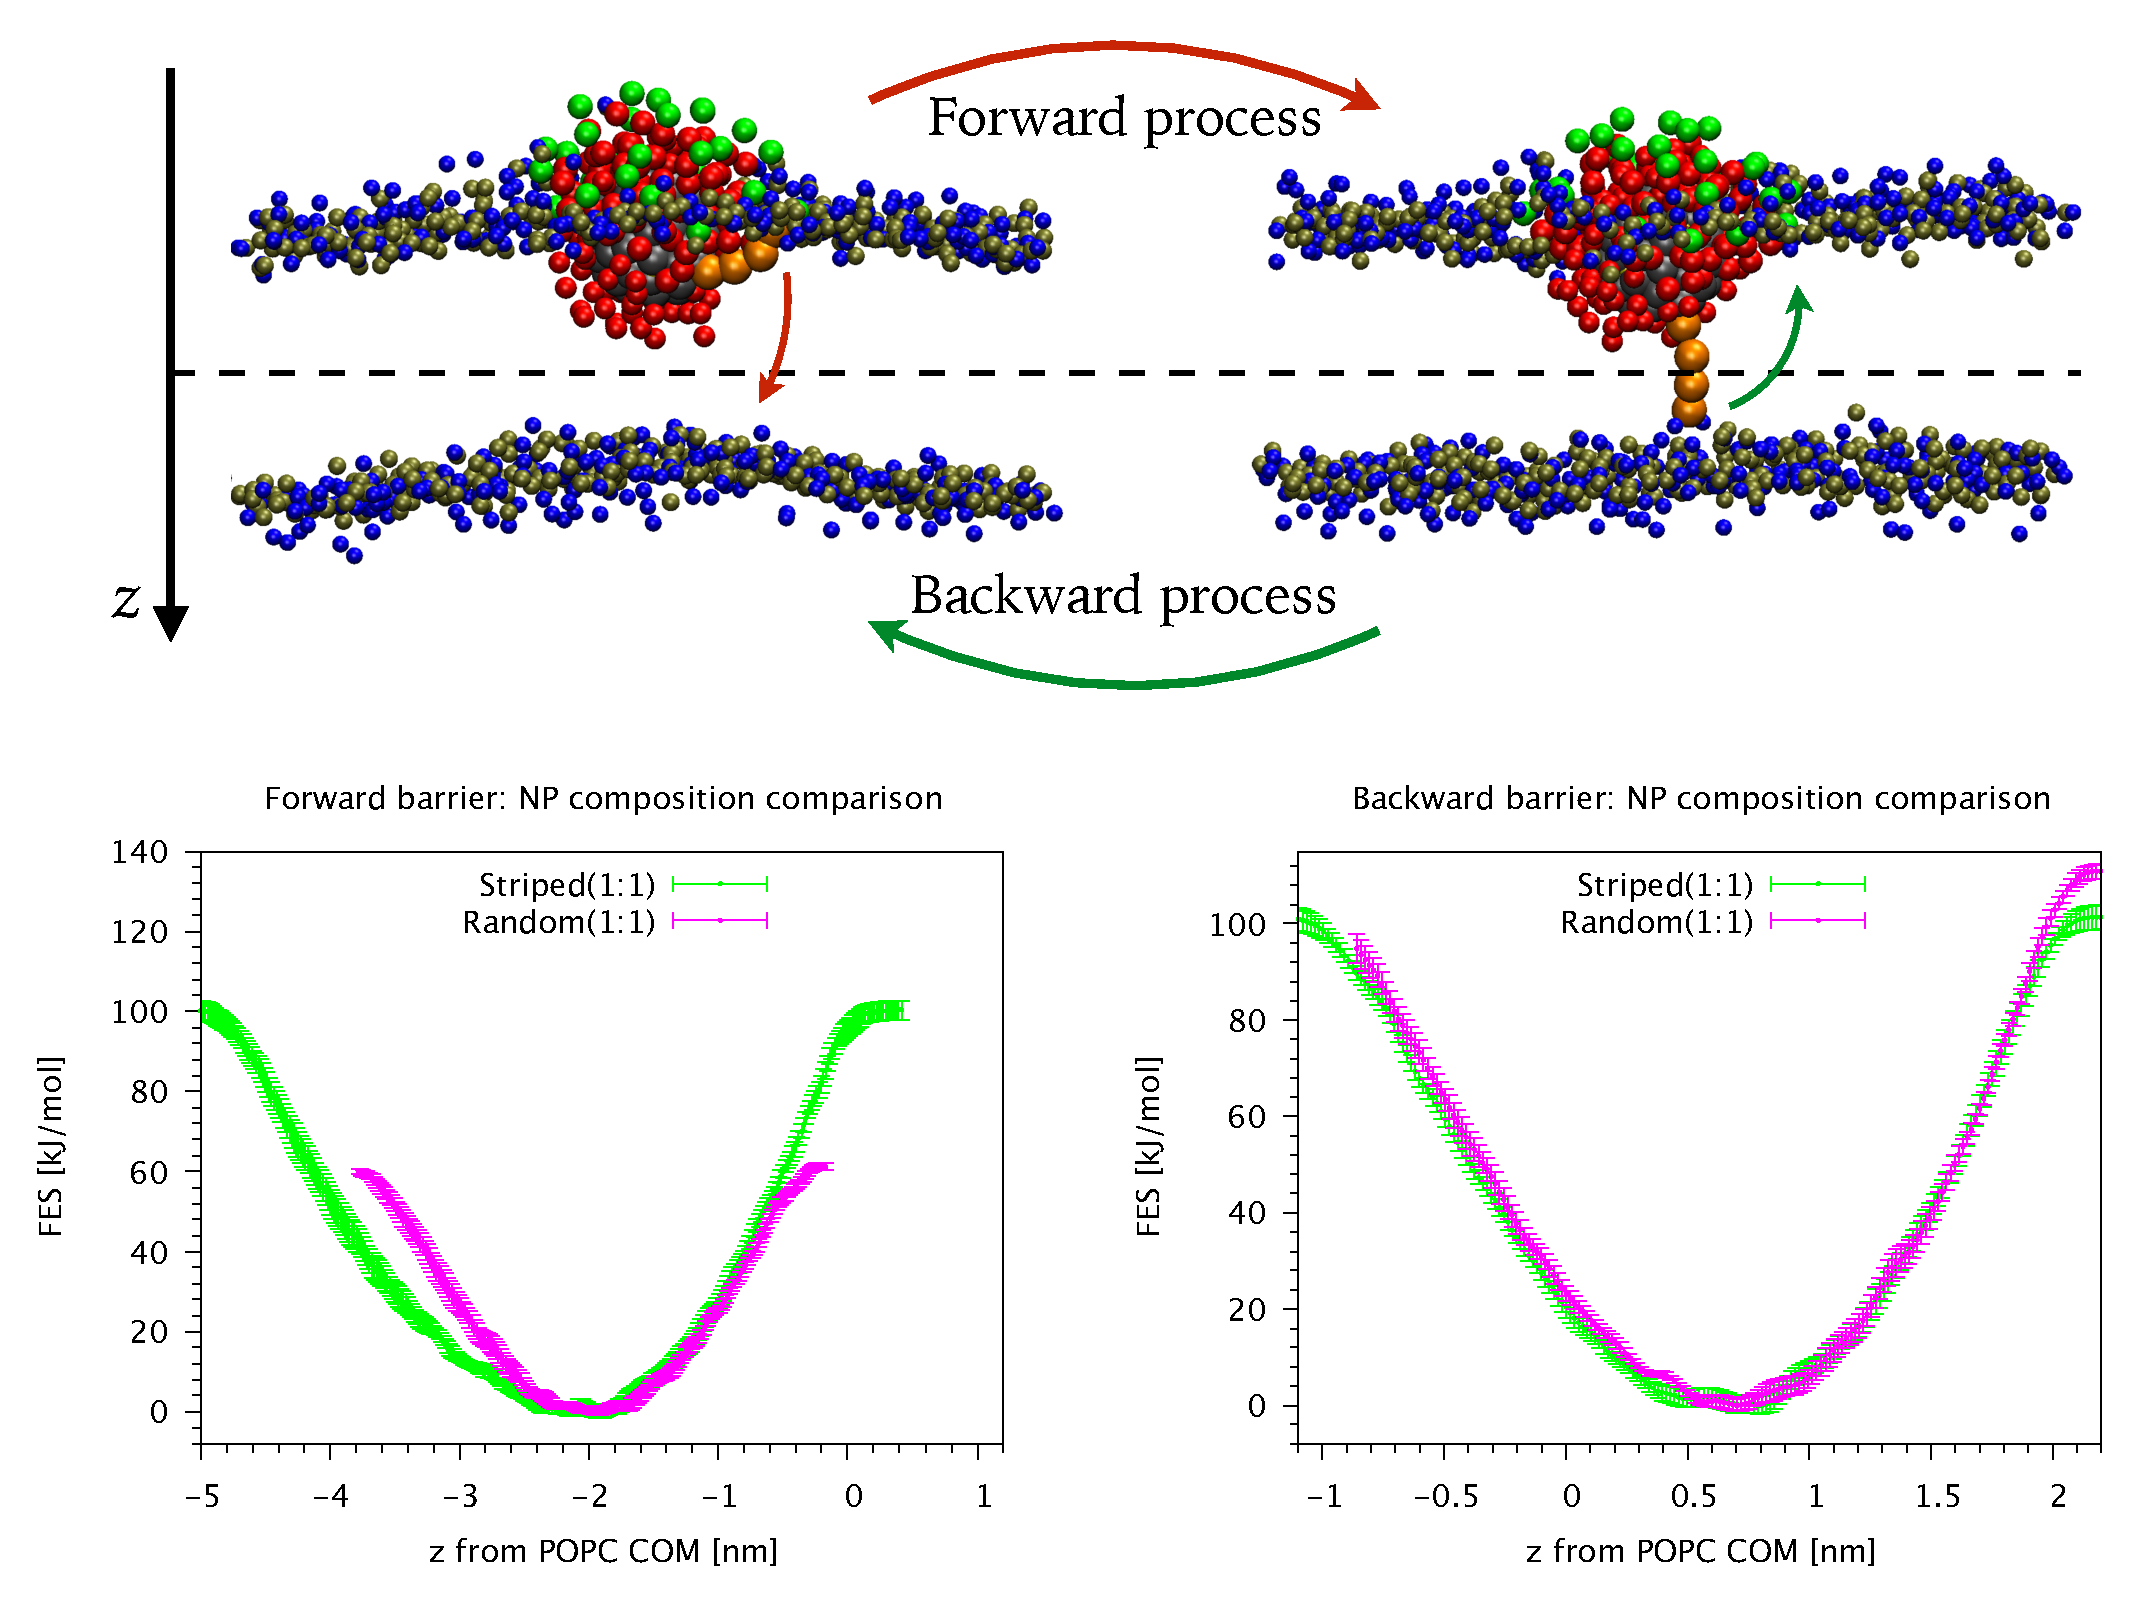
\includegraphics[width=1\textwidth]{./img/coglionazzo}
	\caption{Top: a charged ligand (orange beads) during the membrane translocation process: from the hydrophobic contact in the entrance leaflet to one anchor state in the opposite leaflet, forward process; and \textit{vice versa}, backward process. The dashed line is the \acs{COM} of the bilayer. Water beads and lipid tails are not shown. Color code as in figure~(\ref{fig:NPSummary}). Bottom: the related free energy profiles, separately for the forward (left panel) and the backward process (right panel), for the striped (green curve) and the random (violet curve) \acs{NP}.}%
	\label{fig:coglionazzo}
\end{figure}%
\newpage
	\indent\textit{Future perspectives}. They may consist in more studies of these free energy profiles. In particular, how the free energy profiles of the translocation process depend on the number of ligands already anchored in the anchoring leaflet and if it is helped or hindered by other \acp{NP} embedded in the lipid bilayer. Moreover, we could aim at improving a few technical issues related to the free energy calculations. In particular, the phase space sampling could be made easier using more than a single collective variable during the metadynamics runs.%

 	\item \textbf{\textsf{What model is more appropriate to study charged \ac{NP}--membrane interactions? It is necessary to include long range electrostatic interactions and use a water model that allows for explicit electrostatic screening.}}\\For the striped (\acs{MUS}:\acs{OT} $1$:$1$) \ac{NP} we have compared the free energy profile for the anchoring process obtained with three \ac{CG} models that treat the electrostatic interactions differently. \ac{CG} data have been compared also to atomistic data (Federica Simonelli courtesy). The results are shown in figure~(\ref{fig:forwardWall}). As summarized in table~(\ref{tab:hydroTime}), the free energy barriers for the anchoring process are: $\sim26$~kJ/mol for the \ac{STD} \martini{} model; $\sim36$~kJ/mol with the \ac{PME} method and $\sim134$~kJ/mol for the atomistic one. The \ac{CG} model that best approaches the atomistic result is the \martini{} with both \ac{PME} and the \ac{PW} model with a free energy barrier of $\sim100$~kJ/mol. Thus we conclude that, thanks to its extremely high computational efficiency, \textit{the \ac{STD}} \martini{} \textit{\ac{CG} \ac{FF} remains indispensable for qualitative results} and for understanding the overall molecular mechanism of \ac{NP}--membrane interaction. Quantitatively reliable results should be obtained, even at \ac{CG} level, taking into account long range electrostatics and water polarizability.%

	\item \textbf{\textsf{Can the surface arrangement of ligands influence the \ac{NP} interaction with the membrane? Yes, it can.}}\\As shown in the bottom left panel of figure~(\ref{fig:coglionazzo}), with the best \ac{CG} model, the striped (\acs{MUS}:\acs{OT} $1$:$1$) \ac{NP} (green line) has an anchoring free energy barrier of about $100$~kJ/mol while the random (\acs{MUS}:\acs{OT} $1$:$1$) \ac{NP} (violet line) has an anchoring free energy barrier of about $61$~kJ/mol. Thus, \textit{we have confirmed that the surface arrangement of the \ac{NP} ligands can affect the free energy profiles} involved in the \ac{NP}--membrane interactions and that \textit{the random arrangement can help the anchoring process}, similarly to what was observed with the \ac{STD} \martini{} \ac{CG} \ac{FF} in \cite{ourPaper}.\\\indent\textit{Future perspectives}. Using a larger \acp{NP} could allow to play with a larger variety of surface ligand arrangements. Moreover we could investigate how the free energy profile is affected by a multicomponent lipid membrane, for example adding cholesterol, that increases the rigidity of the membrane; how the free energy profile changes with different degrees of hydrophobicity of the \acp{NP}; how ligands with different length can affect the free energy profiles.%
\end{enumerate}

\vfill
\begin{flushright}
	\textsl{I remember it like it was interesting}\\\smallskip
	\footnotesize\textsc{\sffamily Professor Farnsworth}\ --\ \textsf{Futurama}
\end{flushright}
